\documentclass[12pt]{article}

\usepackage[utf8]{inputenc}
\usepackage[french,activeacute]{babel}
\usepackage[T1]{fontenc}
\usepackage{amsfonts}
\usepackage{hyperref}
\usepackage{graphicx}
\usepackage{wrapfig}
\graphicspath{ {./images/} }

\title{Eulaire, le jeu avec les graphes}
\author{Azizi Marwan \and Coutard Amelia \and Crague Ilian \and Morel Victor \and Bernard Malaurie}

\begin{document}

\maketitle

\section{Le jeu}

\subsection{Présentation}
\textit{Eulaire} est un jeu réalisé sous la direction d'Adrienne Lancelot. Il faut parcourir un graphe en passant exactement une unique fois par chaque arête le composant. Le but est d'enchaîner les niveaux le plus vite possible pour se faire une place dans le classement des meilleurs joueurs du monde  !

\vskip 2cm

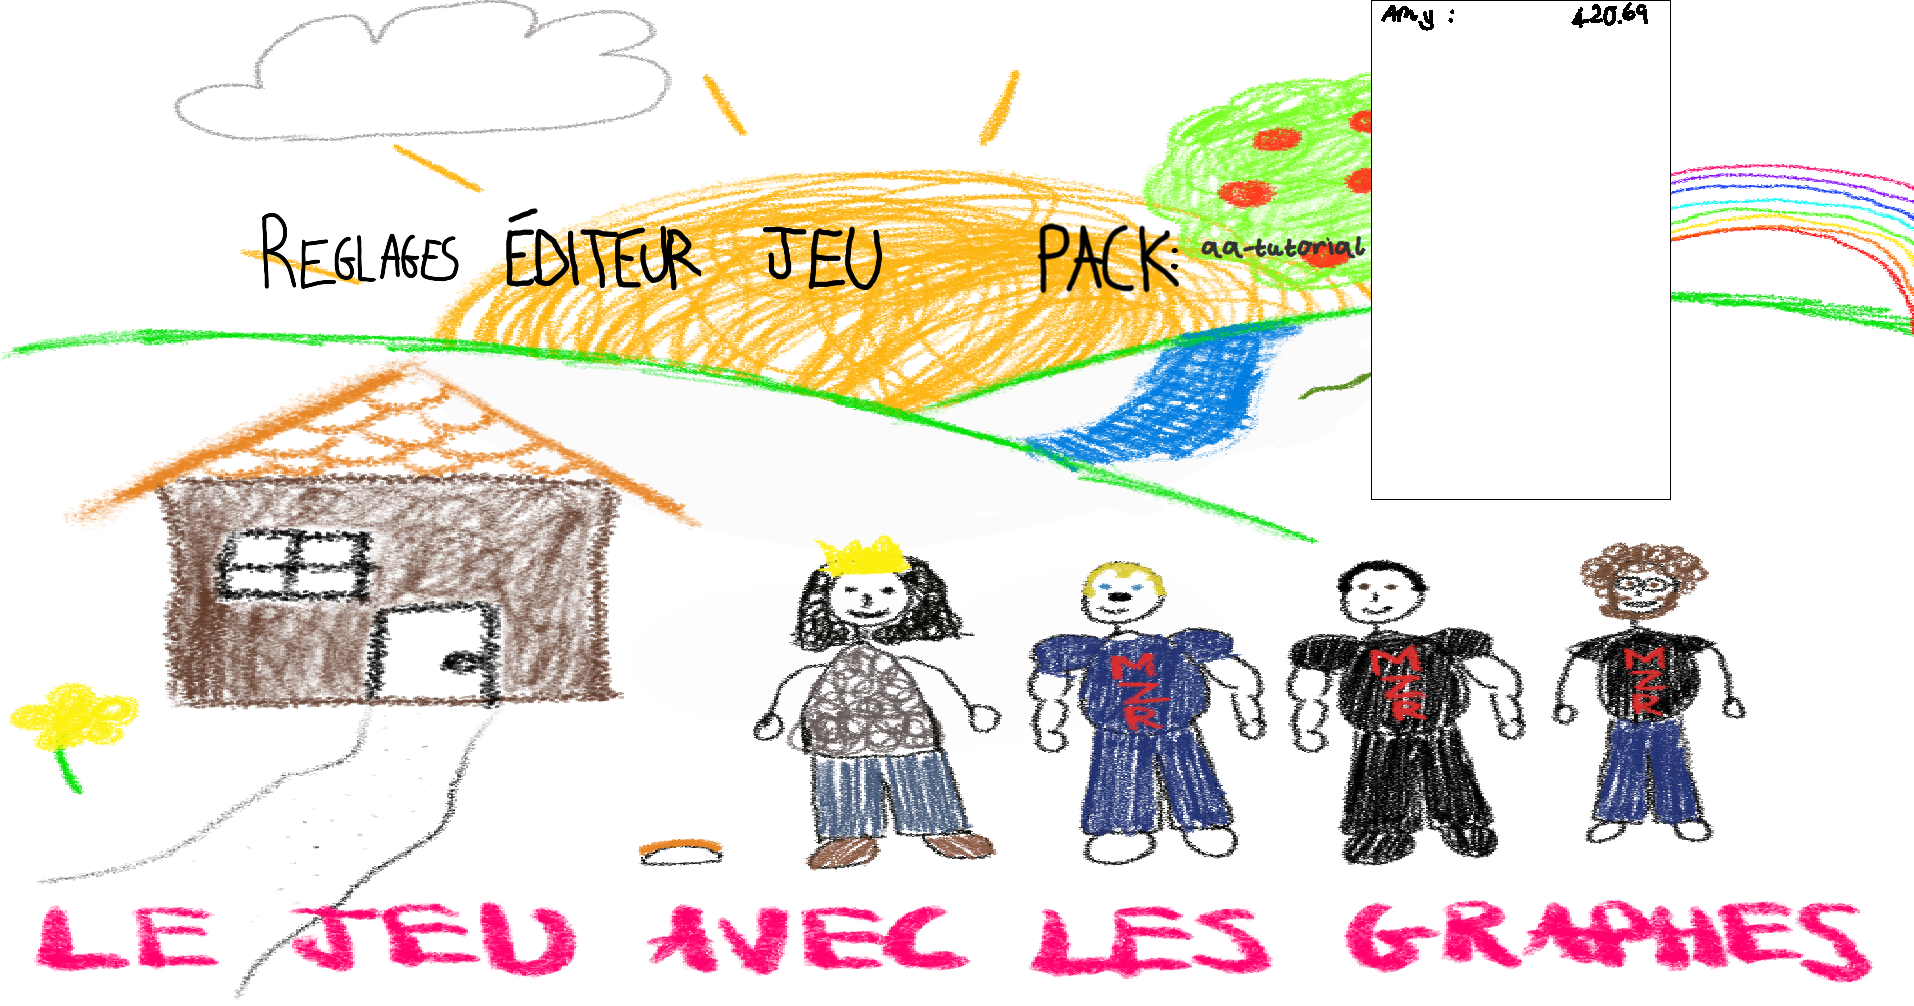
\includegraphics[scale=0.2]{images/menu.png}


\subsection{Lancer le jeu}
Le code source du projet se trouve sur notre dépôt \href{https://gaufre.informatique.univ-paris-diderot.fr/eulaire/2022-al1-ga-eulaire}{gaufre}. Une fois cloné, il suffit d'exécuter \textit{make run} à la racine

\section{Les graphes}
\begin{wrapfigure}{r}{0.2\textwidth}
    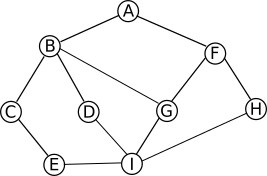
\includegraphics[width=0.25\textwidth]{images/graphe.png}
\end{wrapfigure}

Les graphes ont une place centrale dans notre projet, prétant leur nom à celui de notre jeu, et leur structure étant l'élément principal autour duquel tout le \textit{gameplay} prend place.

\vskip 1cm

\subsection{Qu'est-ce qu'un graphe pour nous ?}
Pour nous, un graphe est simplement un ensemble de sommets reliés par des arêtes non-orientées, qui peuvent relier plusieurs fois deux sommets, et ne peuvent pas relier un sommet avec lui-même. On peut le considérer plus formellement comme une paire $ G = (V, f) $ avec
\vskip 0.25cm
\begin{itemize}
    \item $V$ un ensemble de sommets, communément appelés \textit{noeuds}, ou \textit{vertex}
    \item $f : V^2 \rightarrow \mathbb{N} $ une application symétrique et telle que $\forall x \in V, f(x, x) = 0$.
\end{itemize}

\subsection{Quelle implémentation ?}
Nous avons choisi de travailler sur des graphes non-orientés, dans lesquel un sommet ne peut être relié à lui-même, cela n'apportant rien au jeu.

Durant la phase de développement du projet, nous avons utilisé deux implémentations différentes des graphes. La première consistant à stocker notre graphe comme une liste de noeuds, chaque noeud contenant uniquement la liste des sommets adjacents à ce dernier, avec répétitions si les sommets étaient reliés plusieurs fois entre eux. La seconde implémentation est la matrice d'adjacence, une matrice composée d'entiers, l'élément à l'indice $(i,j)$ de la matrice indiquant le nombre, potentiellement nul, de segments reliant les sommets numérotés $i$ et $j$.

Chaque graphe était stocké en mémoire sous ces deux formes, l'intérêt de ce mode de fonctionnement nous parraissait être de pouvoir choisir l'implémentation la plus adaptée à chaque opération. En effet les deux implémentations ont leurs avantages : dans le cadre de notre jeu, nous sommes amenés à vérifier si il reste des arêtes dans le graphe. Dans le cadre de l'implémentation sous forme de liste, il suffit de parcourir une fois la liste des $n$ noeuds et de vérifier que chaque élément ne possède pas de voisin ($n$ opérations), mais il faut parcourir un peu moins de la moitié de la matrice ($n(n-1)/2$ opérations).
Cependant pour voir si deux sommets d'indices $i$ et $j$ sont reliés, il suffit de regarder la valeur de l'élément à l'indice $(i, j)$ de la matrice (1 opération), alors qu'il faut parcourir tous les noeuds adjacents à un des sommets et voir si l'autre y apparait pour la liste ($n$ opérations, avec $n$ le nombre de sommets adjacents). Nous faisions donc chaque opération de modification du graphe sur les deux implémentations

Nous avons poursuivi de cette façon durant la grande majorité de la phase de développement, et avons fini par abandonner l'implémentation sous forme de liste. En effet il nous a semblé que faire chaque opération sur les deux implémentations n'était pas rentable par rapport au fait d'exécuter chaque opération (dont les plus couteuses) uniquement sur les matrices.

\subsection{Trouver un chemin eulérien}

L'algorithme pour faire ceci est très simple.

Tout d'abord, il faut vérifier que ce chemin existe. Pour cela, il suffit de compter le nombre de segments qui relient chacun des points à d'autres points. S'il y a 0 ou 2 points qui en ont un nombre impair, le graphe est eulérien: un chemin existe. Sinon, il ne l'est pas.

Ensuite, il suffit de partir d'un point (n'importe lequel si aucun point n'a un nombre impair de segments, un de ceux qui en ont un nombre impair sinon), puis de suivre des segments au hasard jusqu'à ce que ce ne soit plus possible (en passant seulement une fois par chaque sommet). Ensuite, tant qu'on n'est pas encore passé par tous les segments, on choisit un sommet par lequel on est déjà passé et qui possède toujours des segments, puis on refait le même procédé: on terminera sur le même sommet, et on pourra donc insérer cette boucle dans le parcours. Une fois qu'il n'y a plus de segments restants, on a fini.

\section{L'éditeur de graphe}
Une fois le graphe implémenté en machine, il faut l'afficher à l'écran. Mais comment faire ?\\
Il est très difficile de déterminer arbitrairement une représentation adaptée au jeu où les sommets sont espacés, les arêtes ne se confondent pas, etc.\\
Nous avons donc choisi d'incorporer au projet un éditeur de graphe, qui permettrait au créateur de niveau de définir le graphe mais aussi de choisir comment il sera affiché.

\subsection{Créer un graphe}
Le but de l'éditeur est de permettre de créer un graphe le plus simplement et le plus directement possible.

\begin{description}
    \item[Placer un sommet]:
    cliquer là où on veut le placer

    \item[Relier plusieurs sommets]:
    cliquer successivement sur les différents sommets pour former un chemin. Le sommet sélectionné apparaît en vert.\\
    On peut cliquer à nouveau sur ce dernier pour le déselectionner. On peut relier plusieurs fois deux sommets.

    \item[Déplacer un sommet]:
    cliquer sur le sommet, en maintenant le clic jusqu'à arriver à la position souhaitée.

    \item[Supprimer un sommet]:
    sélectionner le bouton "supprimer", puis cliquer sur le sommet à supprimer, pour sortir du mode de suppression, cliquer à nouveau sur le bouton "supprimer".

    \item[Supprimer une arête]:
    sélectionner le bouton "supprimer", puis cliquer et maintenir sur un sommet, déplacer le curseur jusqu'au sommet relié dont on veut supprimer la connexion.\\
    On peut supprimer plusieurs arêtes à la suite en maintenant le clic.

\end{description}


\subsection{Fonctionnalités avancées}
Des fonctionnalités supplémentaires ont été ajoutées à l'éditeur pour le compléter.\\
Le but est de faciliter la conception de niveau mais aussi la prise en main de l'éditeur.
\begin{description}
    \item[Supprimer tout]: supprimer tous les sommets et toutes les arêtes.
    
    \item[Graphe random]: générer un graphe avec un nombre d'arêtes et de sommets aléatoire. Les sommets sont également reliés de manière aléatoire.\\
    Le nombre d'arêtes et de sommet peut être ajusté avec leurs boutons respectifs.

    \item[Importer / Exporter]: importer et exporter des graphes réalisés au préalable dans l'éditeur.\\
    Les graphes sont ensuite sauvegardés au format \textit{mzr} (format inventé pour l'occasion), qui contient les coordonnées de chaque sommet ainsi que la matrice d'adjacence.

    \item[Tutoriel]: le tutoriel du jeu, un pack (voir plus bas) spécial, contient un tutoriel pour l'éditeur également.

    \item[Jeu]: on peut tester comment le graphe fonctionne en jeu: pour cela, il suffit de cliquer sur jeu. On peut revenir à l'éditeur en cliquant sur edit.
\end{description}

\section{Réglages}

Des raccourcis ont été ajoutés pour faciliter l'experience des joueurs. Ils permettent de
\begin{itemize}
    \item retourner au menu (Touche <echap> par défaut)
    \item réessayer le graphe actuel (Touche r par défaut)
    \item faire un déplacement évident (si il n'y a qu'un chemin possible) (Touche <espace> par défaut)
\end{itemize}

\begin{description}
    \item[Modifier un réglage] : Pour modifier un réglage, il faut depuis le menu cliquer sur le bouton réglage puis,
    \begin{enumerate}
        \item Cliquer avec la souris sur le réglage à modifier
        \item Cliquer sur la touche du clavier à attribuer
    \end{enumerate}
\end{description}

Aucun test n'est fait pour savoir si le joueur a déjà attribué une touche, on suppose que nos utilisateurs ont un minimum de bon sens.

\section{Le jeu}

\begin{description}
    \item[Principe de base]: le jeu est composé d'un ensemble de packs, qui contiennent chacun plusieurs graphes. Dès que l'on complète un graphe, c'est à dire qu'on trouve un chemin qui passe par toutes les arêtes, le jeu passe automatiquement au graphe suivant. Une fois qu'on a complété tous les graphes, on arrive à un écran de fin, et on peut enregistrer notre score et notre nom. Pour tracer le chemin, on peut cliquer sur les sommets dans l'ordre, ou maintenir le clique et passer sur les sommets dans l'ordre.

    \item[Aide]: on peut obtenir de l'aide: si on clique sur le bouton aide, il nous indique le chemin à suivre, appui par appui. Attention cependant, chaque appui cause une pénalité dans le score final.

    \item[Retry]: il est possible, et même souvent nécessaire, de refaire un graphe car on a fait une erreur: il suffit d'appuyer sur le bouton retry. On peut aussi simplement appuyer sur la touche R.

    \item[Tutoriel]: si on clique sur le bouton jouer sans avoir sélectionné de pack, on se retrouve dans le tutoriel, qui explique comment le jeu et l'éditeur fonctionnent.

    \item[Menu]: pour revenir au menu, il faut et il suffit d'appuyer sur la touche échap.

    \item[Déplacement évident]: si un seul segment est relié au point actuel, il suffit d'appuyer sur espace pour le traverser.
\end{description}

\end{document}
